\paragraph{Example 1}{
\begin{lstlisting}[language=Python]
from BNumMet.Random import clear_mt_vars,genrand
clear_mt_vars()
for i in range(10):
    print(genrand())

>>  Initialized the global dictionary mtVars with seed 4357
    0.8173300600185361
    0.9990608997175147
    0.5103543725587322
    0.13153290984489324
    0.03541634837990076
    0.9924695345089932
    0.6257087035630151
    0.06259194576707482
    0.4107105111262553
    0.13477367491805314
\end{lstlisting}
}
\paragraph{Example 2}{
\begin{lstlisting}[language=Python]
from BNumMet.Random import clear_mt_vars,genrand
clear_mt_vars()
toPlot = [(genrand(),genrand()) for i in range(100000)]
plt.scatter(*zip(*toPlot), s=1, c="black")
\end{lstlisting}
\begin{figure}[H]
    \centering
    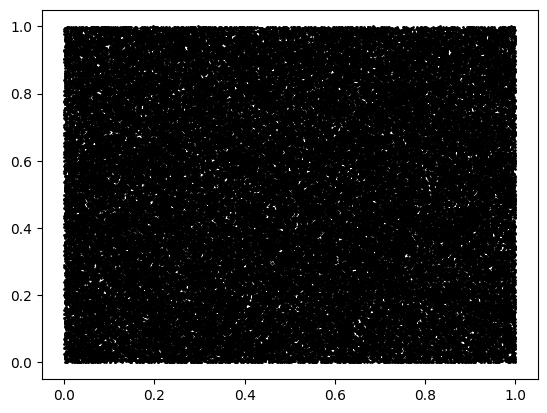
\includegraphics{Include/Images/Thesis/Documentation/Randomness/MersenneTwister Rand Example 2.png}
    \caption{Mersenne Twister Rand Example 2}
    \label{fig:Mersenne Twister Rand Example 2}
\end{figure}
}